
\section{Experiments}
\label{sec:experiments}

\subsection{Experimental Setup}
\label{sec:exp_setup}


\paragraph{World Data}
We design three worlds with distinct social settings to study agents' behaviors in different social environments.
Each world contains 100 uniquely designed agents with diverse backgrounds,
personalities, and initial social relationships.
The details of the world design and character creation are introduced in \S~\ref{app:creation}.
The three worlds are summarized as follows:
\begin{itemize}
  \item \textbf{The Apartment}: a shared-living residential building in New York City,
        inhabited by young professionals, students, and artists.
        It highlights how strangers organically form community bonds
        and relationships within a shared living space.
  \item \textbf{Arcane Academy}: a magical academy setting
        where students and faculty navigate both academic and interpersonal challenges.
        It highlights how complex relationships develop
        within a structured academic institution.
  \item \textbf{The Campus}: a Chinese high school setting,
        centering on student and teacher interactions in a contemporary educational environment.
        It highlights school social network formation
        and personal growth trajectories.
        Its simulation runs in Chinese.
\end{itemize}

\paragraph{Simulation}
We conduct simulations across the three worlds, running for 10 simulated years.
Each simulated year consists of $n_w$ weeks, and each week consists of $n_c$ contact rounds and $n_d$ activity days.

\paragraph{Models}
We use Qwen3.5-397B-A17B~\citep{qwen35} as the primary model
for both the agents and the environment model.
When a model fails to produce valid outputs,
we fall back to Gemini 3 Flash\footnote{\url{https://ai.google.dev/gemini-api/docs/models/gemini-3-flash-preview}} for re-generation.
For more details on generation parameters, see \S~\ref{app:config}.

\paragraph{Metrics}
We track a set of analytical metrics to describe agent behaviors and social dynamics,
covering rewards, fulfillment, activity behaviors, contact behaviors,
personal growth, and computational cost.
Full metric definitions are provided in \S~\ref{sec:appendix_metrics}.


\subsection{Analysis of Long-Term Social Simulation}
\label{sec:long_term_analysis}

\paragraph{Reward Analysis}
We analyze the distribution and temporal trends of the three rewards across
all three 10-year simulations (100 agents $\times$ 10 years $\times$ 3 worlds = 3{,}000 observations).
Figure~\ref{fig:reward_distribution} presents the pooled distributions,
where color intensity indicates agent density
and triangles mark annual means.
Per-world breakdowns are provided in \S~\ref{sec:appendix_reward_per_world}.

\begin{figure*}[htbp]
  \centering
  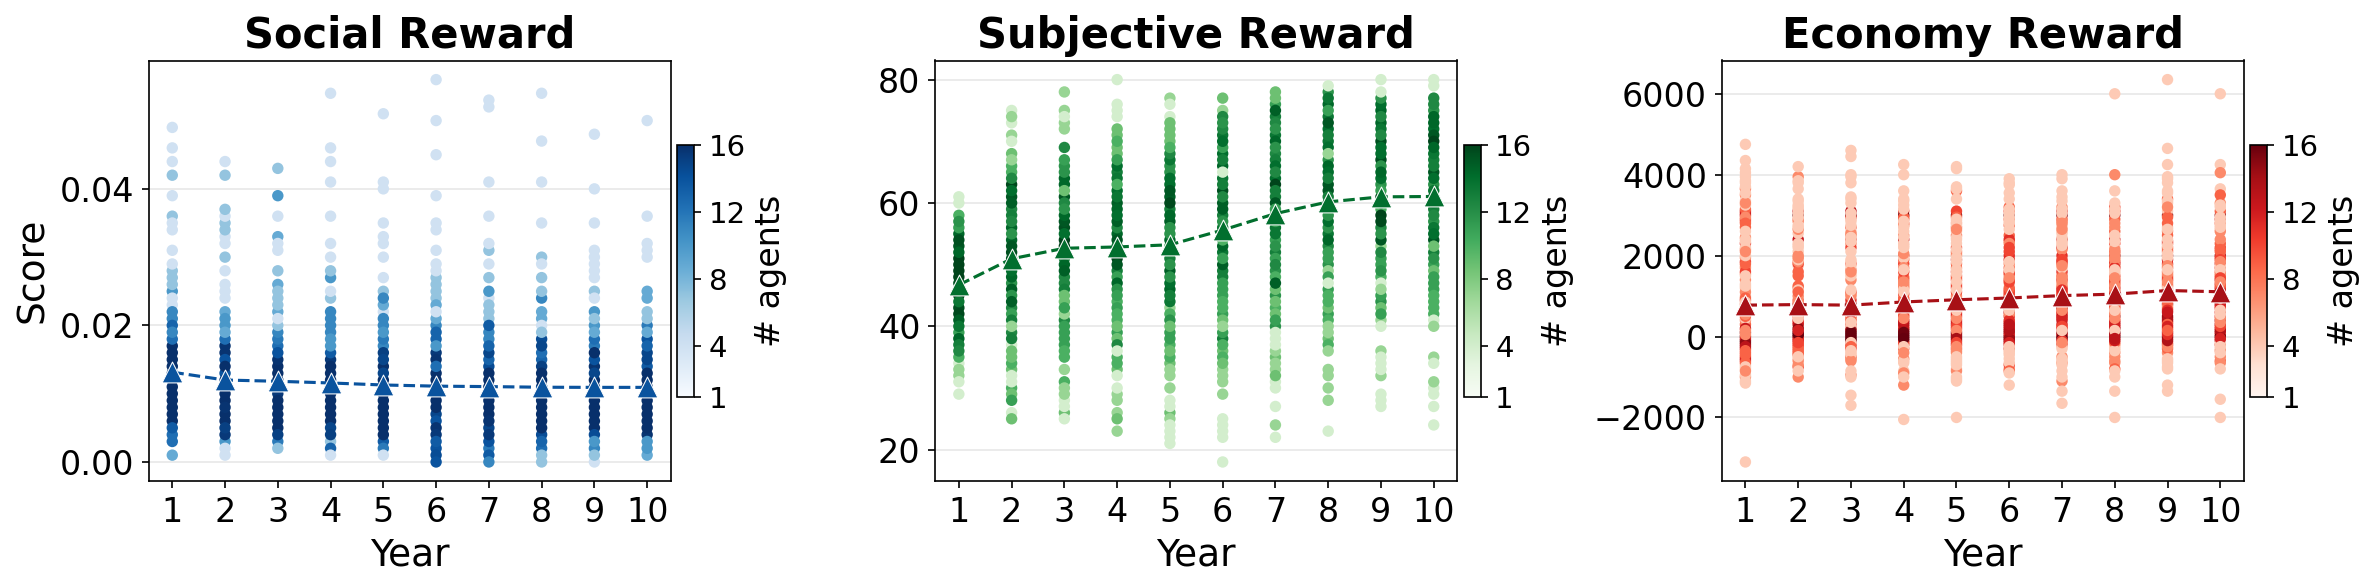
\includegraphics[width=\textwidth]{Figures/reward_distribution_combined.png}
  \caption{%
    Distribution of three reward dimensions over 10 simulated years, pooled across all three worlds.
    Triangles mark annual means.
  }
  \label{fig:reward_distribution}
\end{figure*}

Both subjective and economy rewards show upward trends on average,
while social reward remains broadly stable,
as it is based on agents' relative rankings rather than absolute performance.

\paragraph{Reward--Behavior Correlation}
To understand what drives each reward dimension,
we compute Pearson correlations between behavioral metrics and the three rewards
for each world separately, then average the per-world coefficients to obtain combined values.
Figure~\ref{fig:reward_behavior_correlation} presents the full correlation matrix.


We highlight four findings:
(1) Total reward correlates most strongly with fulfillment dimensions,
social evaluation metrics, and token consumption,
while penalties show the strongest negative signal ($r = -0.50$);
(2) social reward correlates almost exclusively with reputation metrics
(respected by and liked by, $r = 0.68$), which is natural by design; 
it also correlates with numbers of active and passive contacts ($r = 0.09$ and $r = 0.15$)
as well as numbers of proposed and participated joint activities ($r = 0.15$ and $r = 0.19$),
suggesting that agents who engage more in social interactions gain higher social reward;
(3) subjective reward is driven by four fulfillment dimensions by design---mood
($r = 0.54$), material ($r = 0.73$), social ($r = 0.52$), and esteem ($r = 0.30$)---and
unmet fulfillment needs trigger penalties ($r = -0.64$), which substantially reduce subjective reward;
it also correlates with metrics about contacts, joint activities and spending;
(4) economy reward is primarily determined by deposit accumulation ($r = 0.56$)
and extra earning counts, with skills as an indirect positive factor.
Detailed analysis is provided in \S~\ref{sec:appendix_reward_correlation}.
Additional analyses are provided in the appendix, including
friend distribution (\S~\ref{sec:appendix_friend_distribution}),
social network visualization (\S~\ref{sec:appendix_social_network}),
inter-reward correlations (\S~\ref{sec:appendix_reward_correlation_inter}),
wealth inequality (\S~\ref{sec:appendix_matthew_effect}),
reward quartile profiles (\S~\ref{sec:appendix_reward_success_profile}),
striving vs.\ leisurely agent profiles (\S~\ref{sec:appendix_ambition_profile}),
cross-world divergence (\S~\ref{sec:appendix_cross_world}),
and model comparison (\S~\ref{sec:appendix_model_comparison}).

\begin{figure}[htbp]
  \centering
  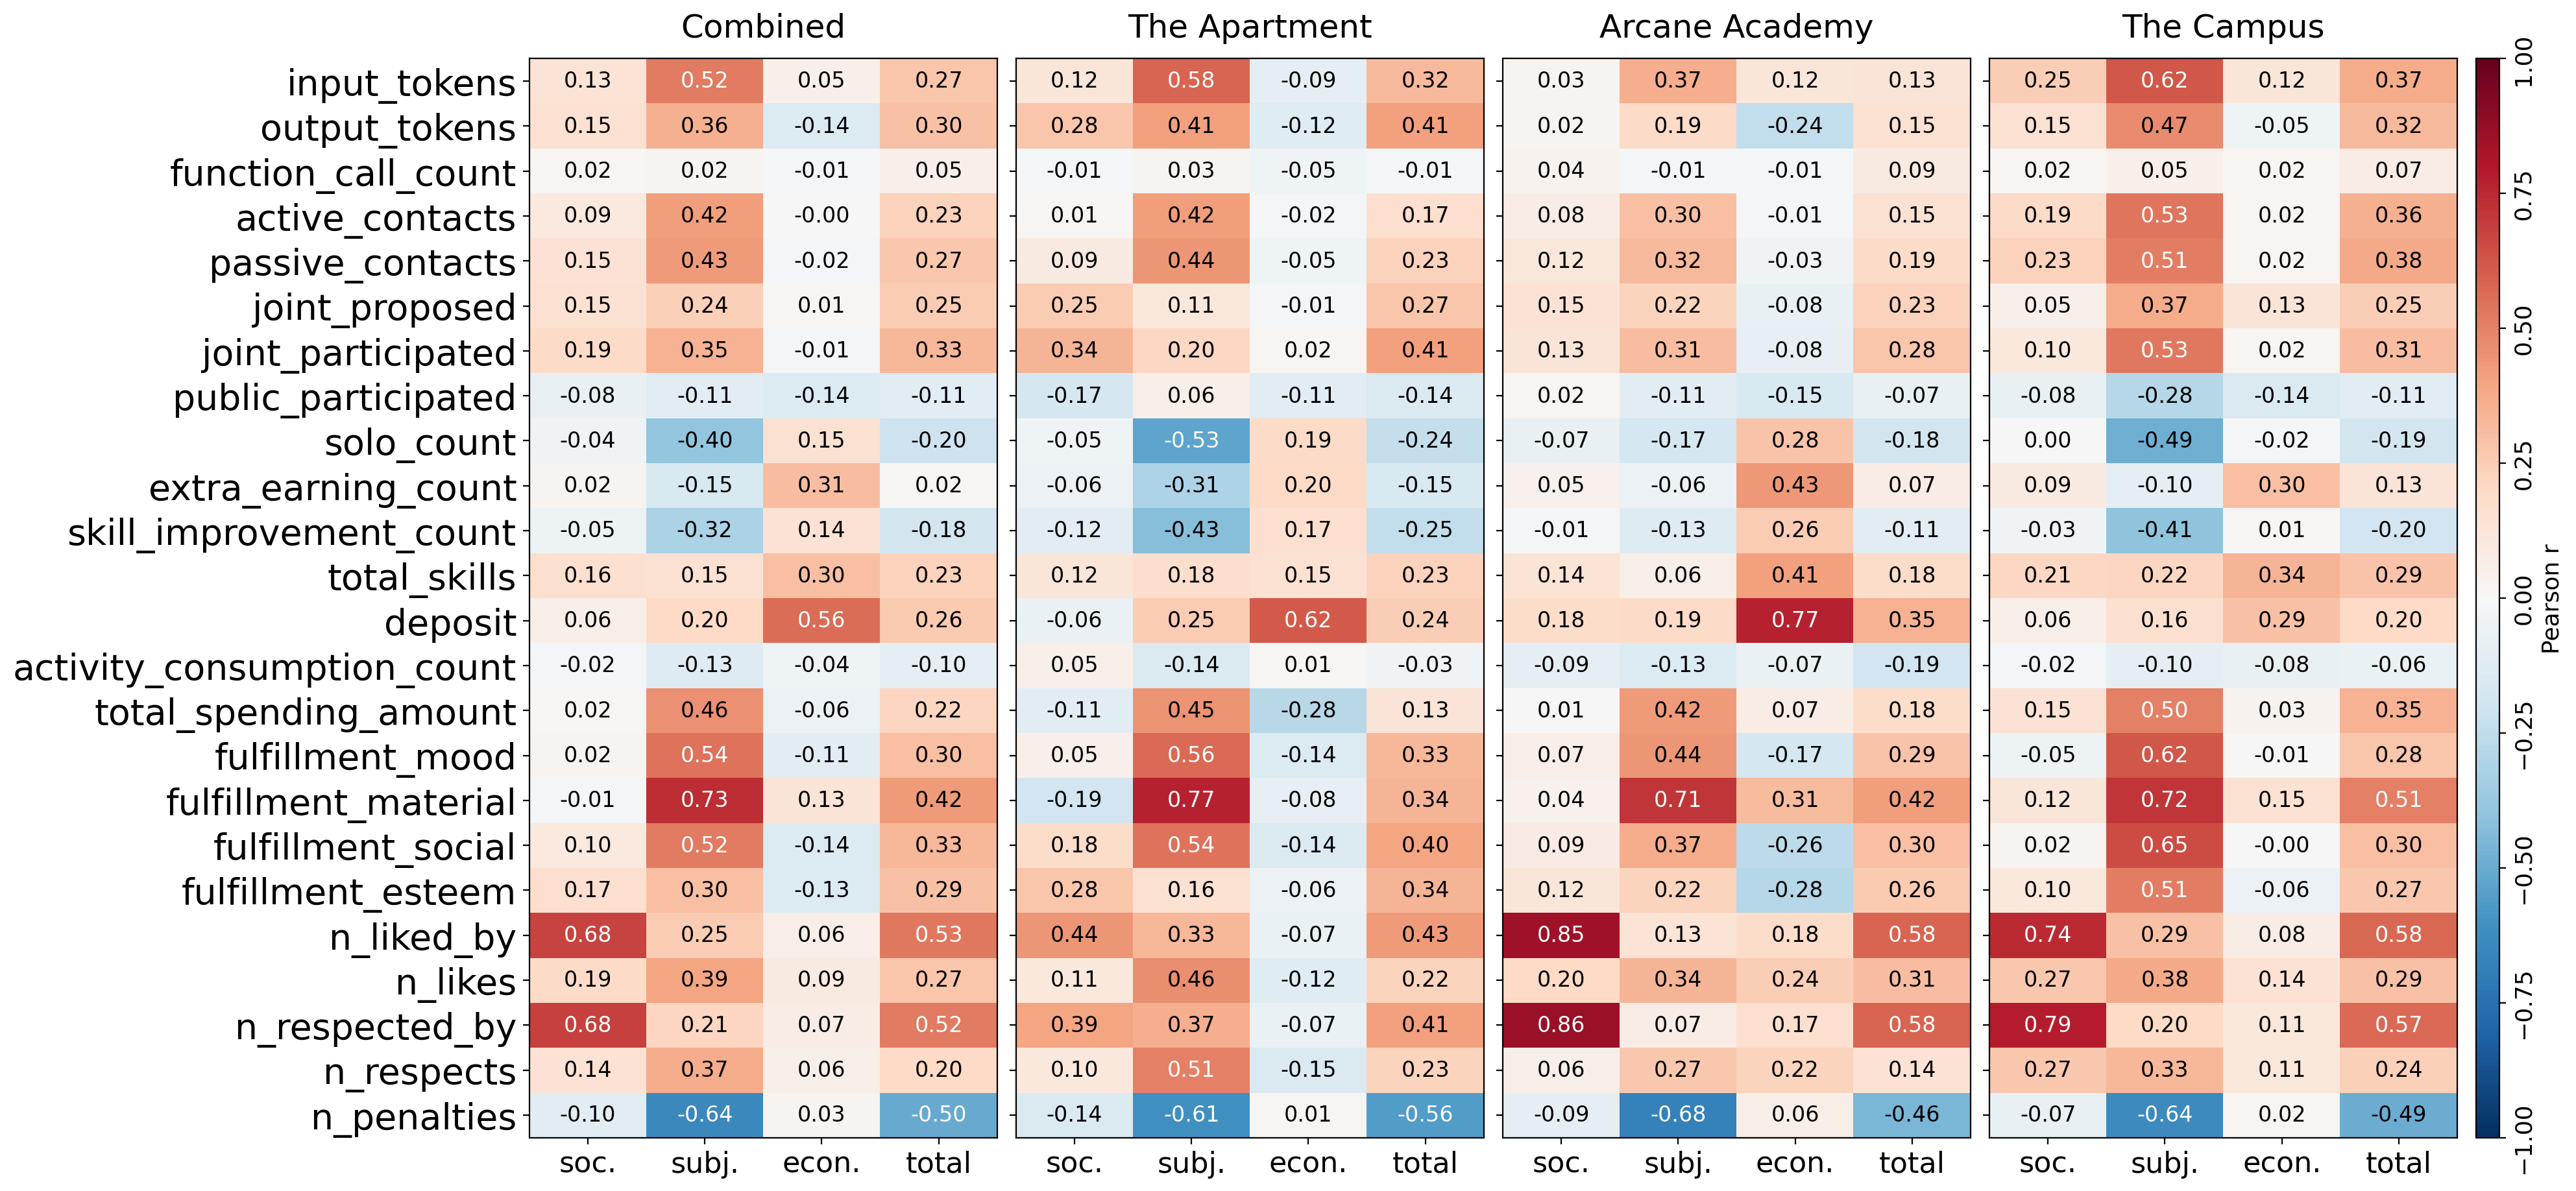
\includegraphics[width=\textwidth]{Figures/reward_behavior_correlation.png}
  \caption{%
    Pearson correlation heatmap between 24 metrics and reward dimensions.
    The \textit{Combined} column averages per-world values.
  }
  \label{fig:reward_behavior_correlation}
\end{figure}

\subsection{Training via Life Rewards}
\label{sec:sft}

\paragraph{Training}
We apply life reward training (\S~\ref{sec:training_data}) to fine-tune Qwen3.5-397B-A17B on simulation data from the first four years across all three worlds.
Training is conducted for 1 epoch on 30 nodes of 8$\times$H100 80GB GPUs with a learning rate of $1 \times 10^{-5}$.
Full training details are provided in \S~\ref{sec:appendix_sft}.
We refer to the fine-tuned model as Qwen3.5-397B-Agentopia.

Qwen3.5-397B-Agentopia is then evaluated via 4-year simulations
on \campus{} and \apartment{},
and compared against the original Qwen3.5-397B baseline
under identical world configurations.

\paragraph{Learning via life rewards improves agent performance in social simulation}
\begin{table}[t]
\caption{%
Qwen3.5-397B-Agentopia vs.\ Qwen3.5-397B: cross-world average metrics over four simulated years on \campus{} and \apartment{}.
Delta shows the percentage change of the four-year average from Qwen3.5-397B to Qwen3.5-397B-Agentopia.}
\label{tab:sft_cross_world}
\centering
\small
\setlength{\tabcolsep}{3pt}
\begin{tabular}{l rrrr rrrr rrr}
\toprule
& \multicolumn{2}{c}{Y1} & \multicolumn{2}{c}{Y2} & \multicolumn{2}{c}{Y3} & \multicolumn{2}{c}{Y4} & \multicolumn{3}{c}{Avg} \\
\cmidrule(lr){2-3} \cmidrule(lr){4-5} \cmidrule(lr){6-7} \cmidrule(lr){8-9} \cmidrule(lr){10-12}
Metric & Base & Tuned & Base & Tuned & Base & Tuned & Base & Tuned & Base & Tuned & Delta \\
\midrule
\multicolumn{12}{l}{\textit{Reward Components}} \\
Economy Reward & 1108 & 1271 & 1092 & 1130 & 1038 & 1006 & 1069 & 1008 & 1077 & 1104 & $\uparrow$\,2.5\% \\
Subjective Reward & 46.0 & 46.7 & 50.1 & 48.4 & 51.5 & 52.6 & 51.9 & 55.3 & 49.9 & 50.8 & $\uparrow$\,1.8\% \\
\midrule
\multicolumn{12}{l}{\textit{Social Evaluation}} \\
Respected By & 7.1 & 6.9 & 9.4 & 11.0 & 10.4 & 14.1 & 11.2 & 15.2 & 9.5 & 11.8 & $\uparrow$\,24.2\% \\
Liked By & 5.2 & 5.1 & 6.9 & 7.5 & 7.4 & 9.3 & 8.1 & 9.9 & 6.9 & 8.0 & $\uparrow$\,15.9\% \\
Mutual Respect & 5.2 & 5.1 & 7.3 & 7.9 & 8.1 & 9.9 & 8.3 & 10.1 & 7.2 & 8.3 & $\uparrow$\,15.3\% \\
Mutual Like & 4.1 & 3.9 & 5.2 & 5.3 & 5.5 & 6.4 & 5.6 & 6.0 & 5.1 & 5.4 & $\uparrow$\,5.9\% \\
\midrule
\multicolumn{12}{l}{\textit{Fulfillment}} \\
Material Fulfill. & 43.7 & 35.6 & 41.4 & 32.4 & 41.8 & 37.2 & 46.0 & 41.8 & 43.2 & 36.8 & $\downarrow$\,$-$14.8\% \\
Mood Fulfill. & 76.9 & 78.3 & 88.3 & 86.9 & 89.1 & 91.4 & 88.7 & 92.8 & 85.8 & 87.4 & $\uparrow$\,1.9\% \\
Social Fulfill. & 59.3 & 60.9 & 66.9 & 69.9 & 63.9 & 73.4 & 64.8 & 75.2 & 63.7 & 69.9 & $\uparrow$\,9.7\% \\
Esteem Fulfill. & 42.3 & 44.1 & 44.0 & 44.4 & 43.8 & 46.4 & 43.6 & 47.2 & 43.4 & 45.5 & $\uparrow$\,4.8\% \\
\midrule
\multicolumn{12}{l}{\textit{Activity Patterns}} \\
Joint Proposed & 6.1 & 6.0 & 6.6 & 5.8 & 6.3 & 6.1 & 6.8 & 6.9 & 6.5 & 6.2 & $\downarrow$\,$-$3.9\% \\
Joint Act. & 12.3 & 12.2 & 13.3 & 11.7 & 12.7 & 12.3 & 13.8 & 14.0 & 13.0 & 12.6 & $\downarrow$\,$-$3.6\% \\
Public Act. & 12.1 & 11.2 & 9.1 & 9.5 & 8.2 & 8.7 & 5.4 & 7.9 & 8.7 & 9.3 & $\uparrow$\,7.1\% \\
Solo Act. & 17.4 & 22.4 & 17.9 & 14.5 & 20.3 & 12.6 & 21.5 & 12.4 & 19.3 & 15.5 & $\downarrow$\,$-$19.8\% \\
Skill Advances & 11.9 & 11.3 & 11.3 & 9.2 & 14.7 & 8.2 & 15.1 & 8.6 & 13.3 & 9.3 & $\downarrow$\,$-$29.6\% \\
\bottomrule
\end{tabular}
\end{table}

Table~\ref{tab:sft_cross_world} summarizes the cross-world average metrics,
from which we observe that:
\begin{inparaenum}[\it (1)]
\item \textbf{Rewards.}
Both economy reward (+2.5\%) and subjective reward (+1.8\%) improve on average,
indicating that life reward training effectively enhances agents' overall well-being in social simulation;
\item \textbf{Social recognition.}
Social reward, being rank-based, remains unchanged when all agents improve uniformly.
We instead examine social evaluation metrics (\S~\ref{sec:appendix_metrics}), which measure absolute social recognition as the numbers of peers who like or respect an agent above a threshold.
The results show that Qwen3.5-397B-Agentopia agents are respected by 24.2\% more peers and liked by 15.9\% more on average,
earning broader recognition and more friendships;
\item \textbf{Fulfillment.}
Mood, social, and esteem fulfillment all improve,
suggesting that trained agents better simulate human needs and need-fulfilling behaviors.
On the other hand, material fulfillment declines ($-$14.8\%),
as the economy reward incentivizes saving over spending,
mirroring the real-life trade-off between consumption and savings;
\item \textbf{Activity patterns.}
Public activity participation rises (+7.1\%),
while solo activities decrease ($-$19.8\%)
and skill advances drop substantially ($-$29.6\%).
This shows that life reward shapes agent behavior, steering agents toward rewarded behavioral patterns, while unrewarded actions may be deprioritized.
\end{inparaenum}
Detailed per-year trends and per-world breakdowns are provided in \S~\ref{sec:appendix_sft_trends}.



\paragraph{Life reward training generalizes to role-playing ability}
Qwen3.5-397B-Agentopia is also evaluated on CoSER Test~\citep{wang2025coser},
a role-playing benchmark that assesses LLMs on given-circumstance acting
derived from classic literary scenarios,
across four dimensions:
Storyline Consistency, Anthropomorphism, Character Fidelity, and Storyline Quality.
It is compared against several state-of-the-art open-source and proprietary models,
using Qwen3-235B~\citep{qwen3} as the judge model
(see \S~\ref{sec:appendix_coser} for details).
As shown in Table~\ref{tab:coser_results},
Qwen3.5-397B-Agentopia achieves significant improvements over the baseline Qwen3.5-397B
and outperforms Claude-4.5-Sonnet,
with the most notable gains in Anthropomorphism (+23.7\%) and Character Fidelity (+16.4\%).
This indicates that training with life rewards does not merely optimize agents within \method,
but also improves general anthropomorphism and role-playing capabilities.


\begin{table}[t]
\caption{%
Performance of various LLMs on CoSER Test, judged by Qwen3-235B.
}
\label{tab:coser_results}
\centering
\small
\setlength{\tabcolsep}{3pt}
\begin{tabular}{l ccccccc}
\toprule
& \makecell{Claude\\4.5-Opus} & \makecell{Gemini\\3-Pro} & \makecell{Qwen3.5\\397B-Agentopia} & \makecell{Claude\\4.5-Sonnet} & \makecell{Qwen3.5\\397B} & \makecell{CoSER\\70B} & \makecell{GPT-5\\Mini} \\
\midrule
Storyline Consistency & 63.74 & 65.95 & 41.02 & 47.18 & 39.60 & 35.05 & 38.10 \\
Anthropomorphism      & 64.28 & 60.42 & 49.67 & 36.02 & 40.16 & 31.16 & 24.60 \\
Character Fidelity    & 58.45 & 58.34 & 46.93 & 47.55 & 40.32 & 32.28 & 27.20 \\
Storyline Quality     & 63.24 & 62.49 & 59.01 & 50.09 & 49.97 & 45.33 & 42.00 \\
\midrule
Average               & 62.43 & 61.80 & 49.16 & 45.21 & 42.51 & 35.95 & 32.97 \\
\bottomrule
\end{tabular}
\end{table}

\subsection{Computational Cost}
\label{sec:cost}


\begin{table}[t]
\centering
\caption{Overall cost for three simulation worlds.
Each world runs 100 agents for 10 simulated years.
M = million tokens, K = thousand calls, h = wall-clock hours.}
\label{tab:cost_overall}
\small
\begin{tabular}{l rrrrr}
\toprule
\textbf{World} & Input (M) & Output (M) & Tokens (M) & Calls (K) & Time (h) \\
\midrule
\campus{}       & 19,041 & 425 & 19,466 & 544 & 201.3 \\
\academy{}      & 11,302 & 315 & 11,617 & 572 & 174.2 \\
\apartment{}    &  9,699 & 317 & 10,016 & 584 & 183.2 \\
\midrule
\textbf{Average} & 13,347 & 352 & 13,700 & 567 & 186.2 \\
\bottomrule
\end{tabular}
\end{table}

\begin{figure}[h]
\centering
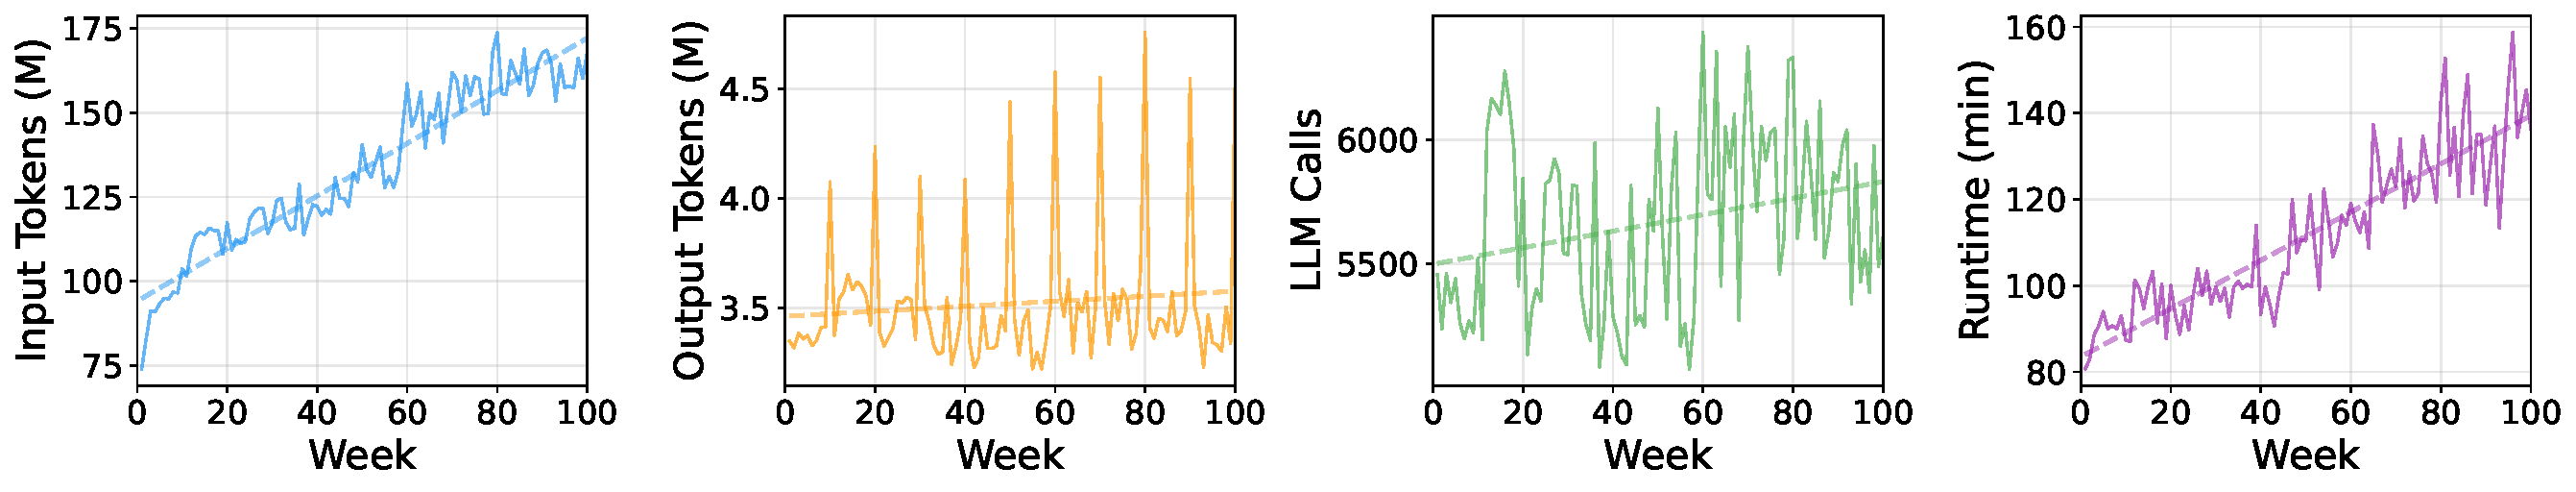
\includegraphics[width=\textwidth]{Figures/cost_trend.pdf}
\caption{Per-week cost trends averaged across three worlds over 10 simulated years.
Dashed lines indicate linear trend fits.}
\label{fig:cost_trend}
\end{figure}

We deploy three FP8 instances of Qwen3.5-397B for each simulation run.
Table~\ref{tab:cost_overall} summarizes the overall cost
for simulating 100 agents over 10 years in each world,
and Figure~\ref{fig:cost_trend} illustrates the per-week cost trends
averaged across three worlds.

On average, a single 10-year simulation consumes 13.7 billion tokens
across 567K LLM calls, completing in approximately 186 wall-clock hours.
Input tokens dominate the cost,
averaging 133M per week compared to only 3.5M for output tokens,
reflecting the heavy context required for each agent's persona and memory.
Both input tokens and runtime increase steadily over time
as agents accumulate memory and context grows,
with per-week runtime rising from approximately 80 to 140 minutes
over the 10-year span.
This indicates that memory growth serves as a major computational bottleneck for long-horizon social simulation, which makes effective context and memory management strategies essential.     
Detailed per-world breakdowns are provided in \S~\ref{sec:appendix_cost}.

